\documentclass[10pt,a4paper,oneside]{article}
\usepackage{cmap}
\usepackage[T2A]{fontenc}
\usepackage{float}
\usepackage{listings}
\usepackage{csquotes}
\usepackage[utf8]{inputenc}
\usepackage{amsmath}
\usepackage{amsfonts}
\usepackage{amssymb}
\usepackage[english, russian]{babel}%Подключаем русский язык.
\usepackage{graphicx}
\usepackage{geometry} % Меняем поля страницы.
\geometry{left=3cm} %Левое поле.
\geometry{right=2cm} %Правое поле.
\geometry{top=3cm} %Верхнее поле.
\geometry{bottom=2cm} %Нижнее поле.


%Начало документа
\begin{document}

%Создаём титульник.
\begin{titlepage}
\newpage
	%Название ВУЗа и институт.
	\begin{center}
		\Large Санкт-Петербургский Государственный Политехнический Университет\\
		Институт Компьютерных Наук и Технологий\\
	\end{center}
	%Кафедра.
	\begin{center}
		\large\textbf {Высшая школа интеллектуальных систем и суперкомпьютерных технологий}
	\end{center}
	
	%Пропуск места. 
	\vspace{5em}
	%!!!!!!!!!!!!!!!!!!!!!!!!!!!!!!!!!Название работы.
	\begin{center}
		\large{Отчёт по лабораторной работе №6 \\ на тему \\
		\textbf{Дискретное косинусное преобразование} }
	\end{center}
	
	%Делаем пропуск и пишем студента и преподавателя.
	\vspace{25em}
	\begin{flushright}
		\textbf{Работу выполнил\\}Студент группы 3530901/80203 \\ Тарасенко Н.С.\\
		\textbf{Преподаватель\\}Богач Н.В. 
	\end{flushright}
	
	\vspace{\fill}%В самом низу
	\begin{center}
	Санкт-Петербург, 2021 год	
	\end{center}
\end{titlepage} %Закончили титульный лист.

\section{Настройка проекта}
Перед тем как выполнять задания необходимо настроить проект и сделать все необходимые импорты:

\begin{figure}[H]
        \centering
        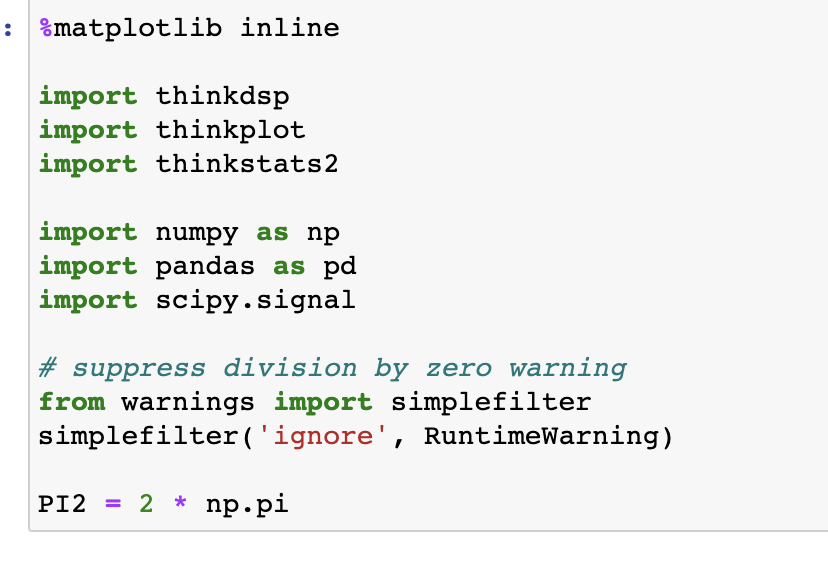
\includegraphics[width=0.75\textwidth]{0.png}
        \caption{2}
        \label{fig:first}
\end{figure}

\section{Упражнение номер №1}

Убедиться, что analyze1 требует времени пропорционально n^3, а analyze2 пропорционально n^2.

Начнём с шумового сигнала и массива величин степени двойки:

\begin{figure}[H]
        \centering
        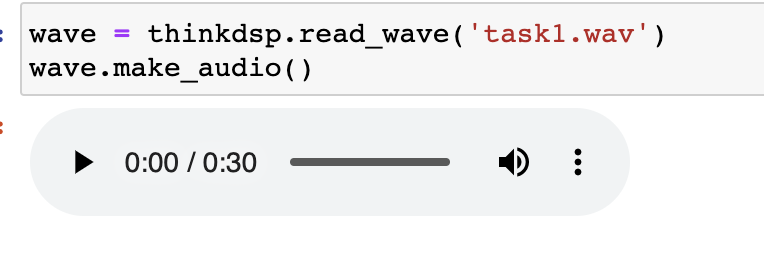
\includegraphics[width=0.75\textwidth]{1.png}
        \caption{2}
        \label{fig:first}
\end{figure}

Следующая функция берет массив результатов временного эксперимента, отображает результаты и выстраивает прямую линию.

\begin{figure}[H]
        \centering
        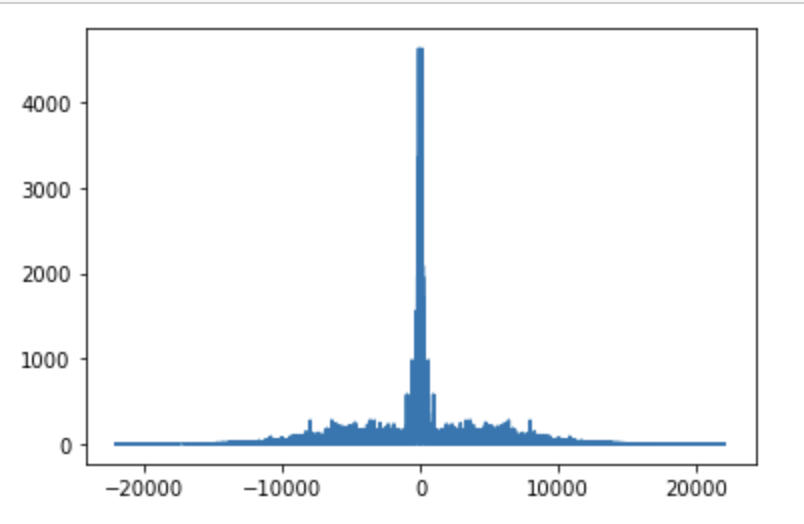
\includegraphics[width=0.75\textwidth]{2.png}
        \caption{2}
        \label{fig:first}
\end{figure}

Выведем результаты для analyze1:

\begin{figure}[H]
        \centering
        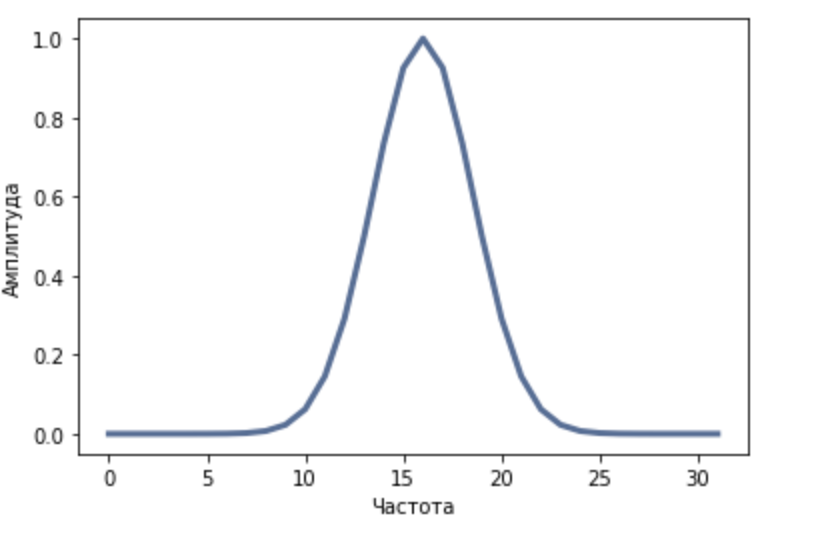
\includegraphics[width=0.75\textwidth]{3.png}
        \caption{2}
        \label{fig:first}
\end{figure}

Расчетный наклон близок к 2, а не к 3, как ожидалось. Одна из возможностей состоит в том, что производительность np.linalg.solve почти квадратична в этом диапазоне размеров массива.

Выведем результаты для analyze2:

\begin{figure}[H]
        \centering
        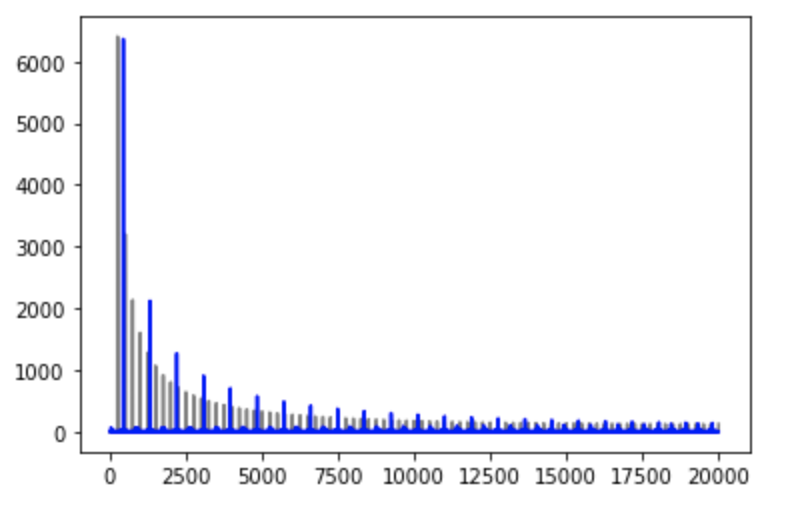
\includegraphics[width=0.75\textwidth]{4.png}
        \caption{2}
        \label{fig:first}
\end{figure}

Как и ожидалось, результаты для analysis2 попадают в прямую линию с предполагаемым наклоном, близким к 2.

Вот результаты для scipy.fftpack.dct

\begin{figure}[H]
        \centering
        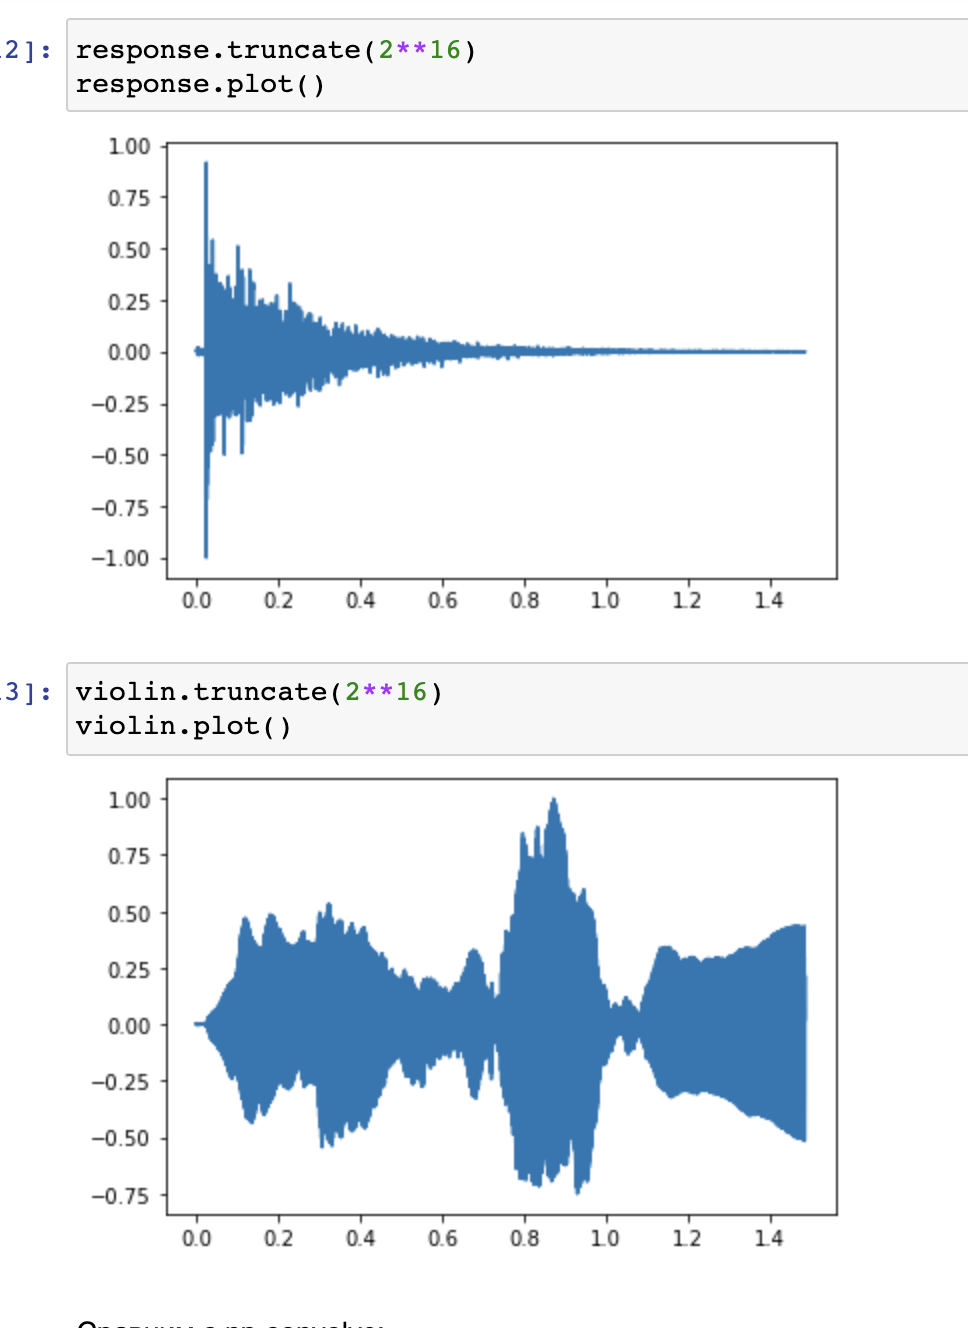
\includegraphics[width=0.75\textwidth]{5.png}
        \caption{2}
        \label{fig:first}
\end{figure}

Эта реализация dct еще быстрее. Линия изогнута, что означает, что либо мы еще не видели асимптотическое поведение, либо асимптотическое поведение не является простым показателем. Фактически, как мы скоро увидим, время выполнения пропорционально logn.

На следующем рисунке показаны все три кривые на одних и тех же осях.

\begin{figure}[H]
        \centering
        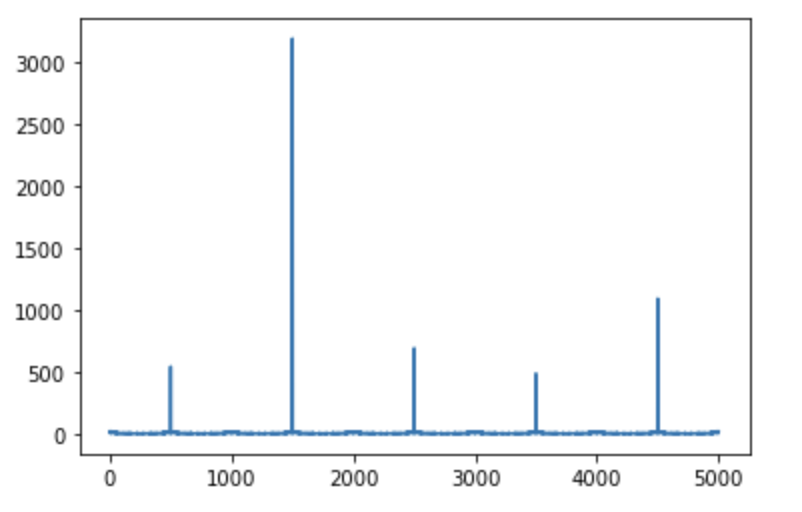
\includegraphics[width=0.75\textwidth]{6.png}
        \caption{2}
        \label{fig:first}
\end{figure}

\section{Упражнение номер №2}

Реализовать алгоритм описанный в учебнике в данной главе. Проверить на записи сколько можно компонентов удалить до того как разница станет заметной. 

thinkdsp предоставляет класс Dct, похожий на Spectrum, но использующий DCT вместо FFT.

Возьмем запись саксофона из репозитория, выделим небольшой сегмент, построим DCT этого сегмента:

\begin{figure}[H]
        \centering
        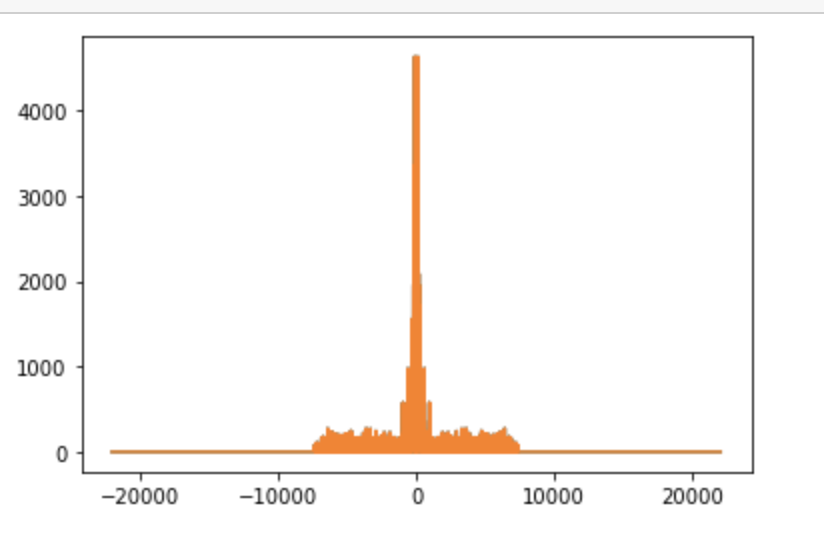
\includegraphics[width=0.75\textwidth]{7.png}
        \caption{2}
        \label{fig:first}
\end{figure}

Есть только несколько гармоник со значительной амплитудой, и многие записи близки к нулю.

Следующая функция принимает DCT и устанавливает для элементов ниже порога значение 0.

\begin{figure}[H]
        \centering
        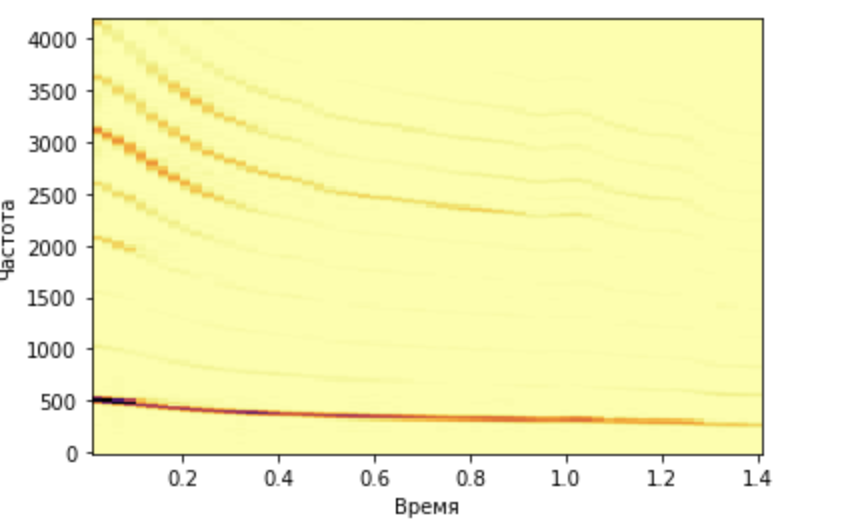
\includegraphics[width=0.75\textwidth]{8.png}
        \caption{2}
        \label{fig:first}
\end{figure}

Если мы применим его к сегменту, мы можем удалить более 90 процентов элементов:

\begin{figure}[H]
        \centering
        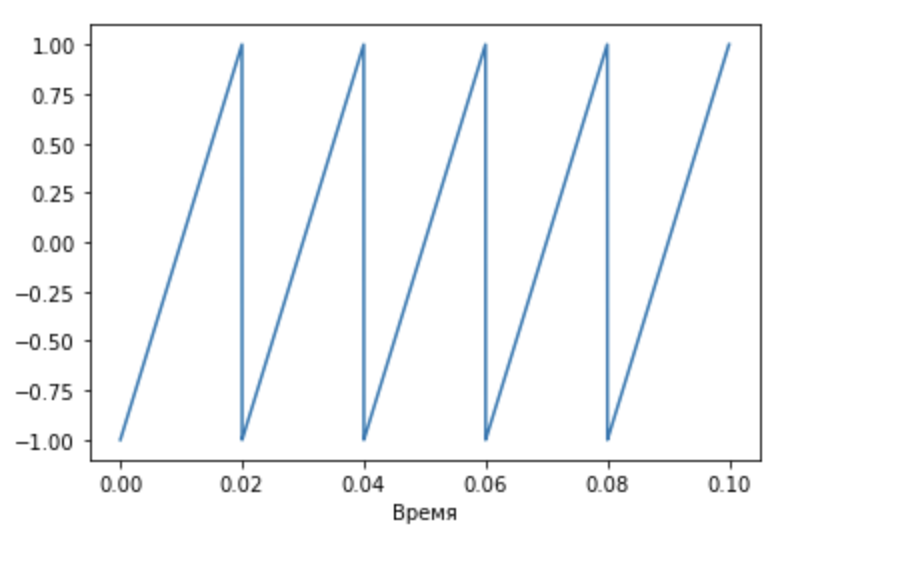
\includegraphics[width=0.75\textwidth]{9.png}
        \caption{2}
        \label{fig:first}
\end{figure}

Результат схож с изначальным

Чтобы сжать более длинный сегмент, мы можем сделать спектрограмму ДКП. Следующая функция похожа на wave.make_spectrogram за исключением того, что использует ДКП.

\begin{figure}[H]
        \centering
        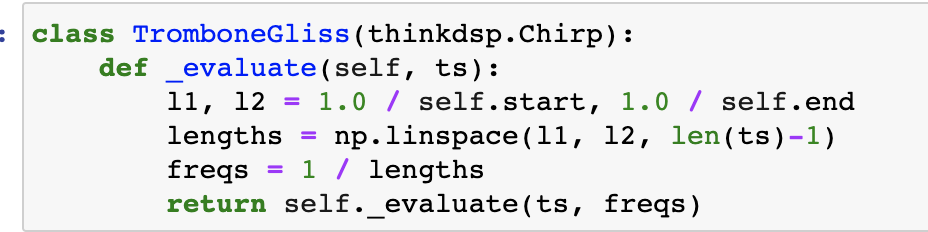
\includegraphics[width=0.75\textwidth]{10.png}
        \caption{2}
        \label{fig:first}
\end{figure}

Теперь мы можем составить DCT-спектрограмму и применить компресс к каждому сегменту:

\begin{figure}[H]
        \centering
        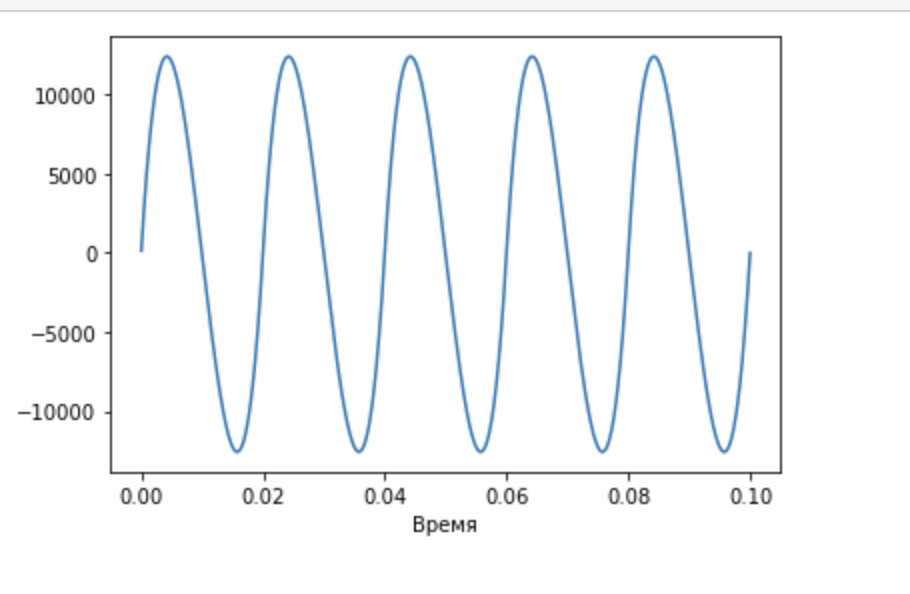
\includegraphics[width=0.75\textwidth]{11.png}
        \caption{2}
        \label{fig:first}
\end{figure}

В большинстве сегментов сжатияие составляет 75-80 процентов.

Чтобы услышать, как это звучать, мы можем преобразовать спектрограмму обратно в волну и воспроизвести ее. При сжатии слышно характерный треск во время воспроизведения аудио, так что можно смело сказать, что нам удалось сжать аудиозапись.

\section{Упражнение номер №3}

Изучить блокнот phase.ipynb

Используем сигнал с пилообразной формой волны. Выведем спектр: 

\begin{figure}[H]
        \centering
        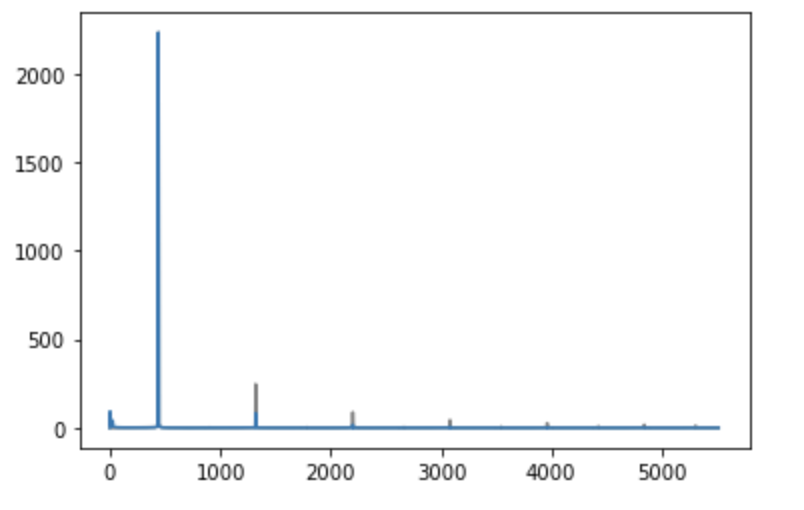
\includegraphics[width=0.75\textwidth]{12.png}
        \caption{2}
        \label{fig:first}
\end{figure}

Рассмотрим угловую часть спектра.

\begin{figure}[H]
        \centering
        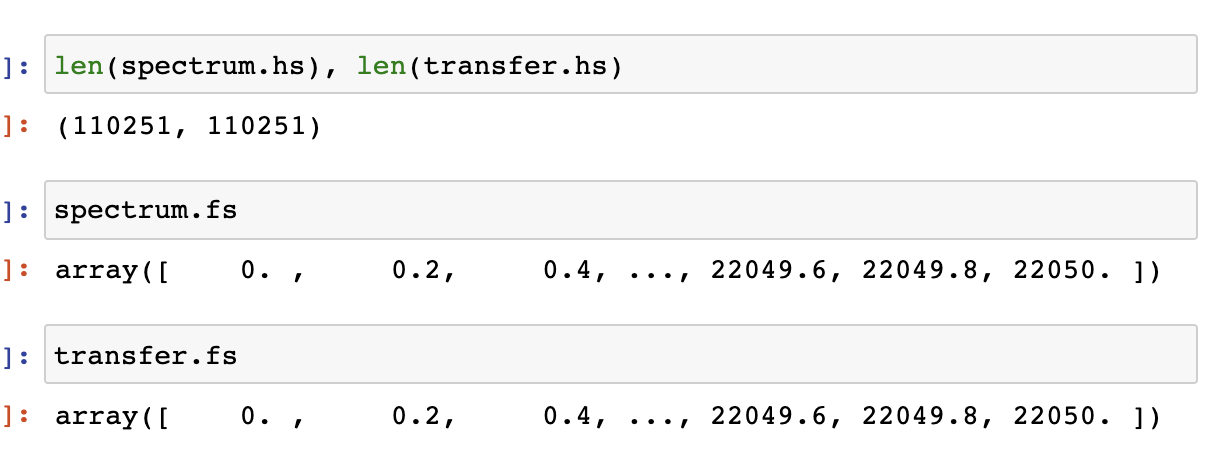
\includegraphics[width=0.75\textwidth]{13.png}
        \caption{2}
        \label{fig:first}
\end{figure}

Когда мы выбираем только те частоты, где величина превышает пороговое значение, мы видим, что в углах есть структура. Каждая гармоника смещена от предыдущей на доли радиана.

Следующая функция отображает амплитуды, углы и форму волны для заданного спектра.

\begin{figure}[H]
        \centering
        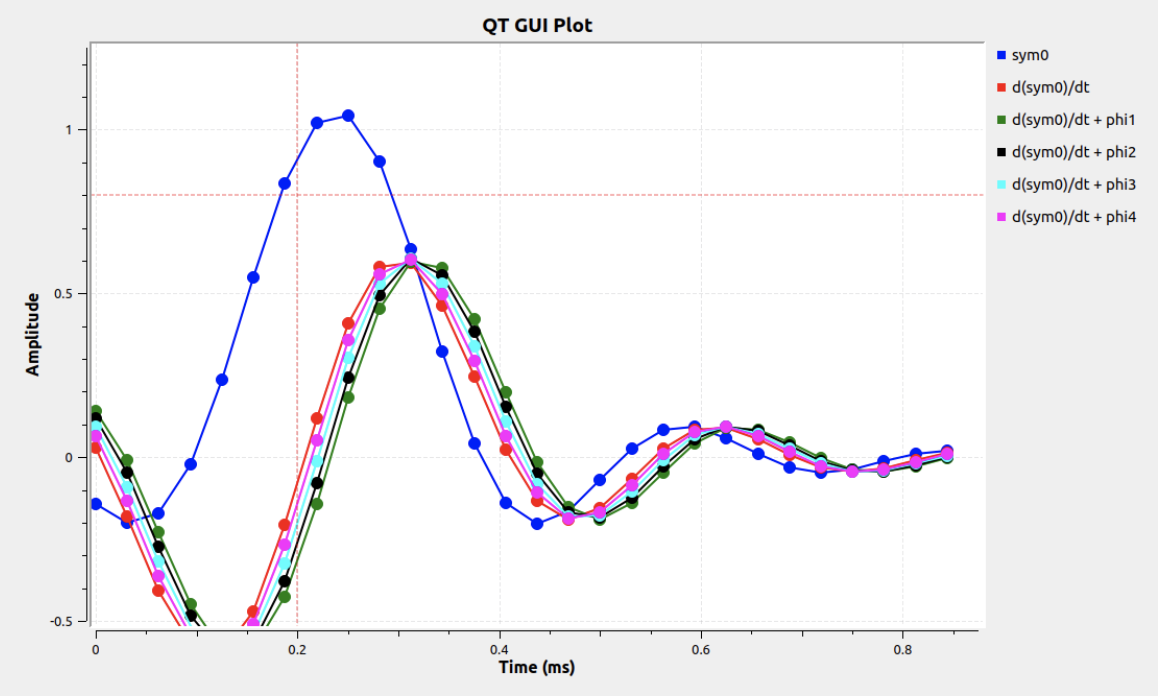
\includegraphics[width=0.75\textwidth]{14.png}
        \caption{2}
        \label{fig:first}
\end{figure}

С помощью функции отобразим неизмененный спектр

\begin{figure}[H]
        \centering
        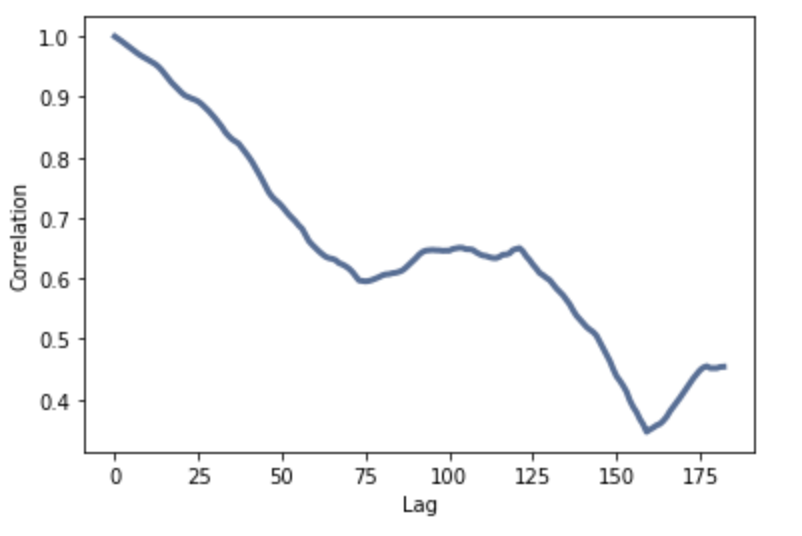
\includegraphics[width=0.75\textwidth]{15.png}
        \caption{2}
        \label{fig:first}
\end{figure}

Рассмотрим ситуация когда все углы устанавливаются в 0, для этого напишем метод позволяющий это сделать.

\begin{figure}[H]
        \centering
        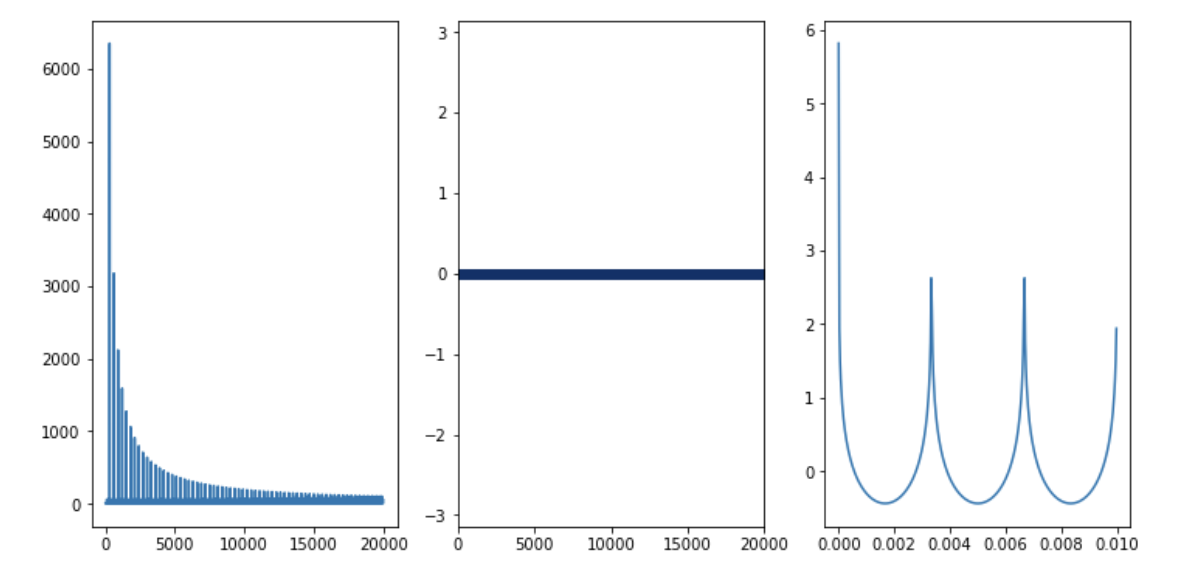
\includegraphics[width=0.75\textwidth]{16.png}
        \caption{2}
        \label{fig:first}
\end{figure}

Если мы умножим комплексные компоненты на exp(iф) , это приведет к добавлению ф к углам:

\begin{figure}[H]
        \centering
        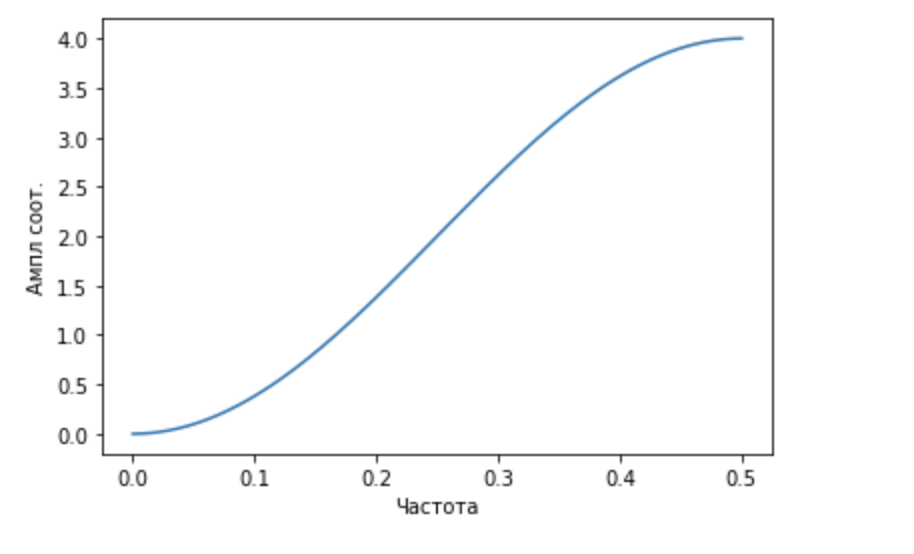
\includegraphics[width=0.75\textwidth]{17.png}
        \caption{2}
        \label{fig:first}
\end{figure}

Рассмотрим ситуация когда все углы устанавливаются в случайные значения, для этого напишем метод позволяющий это сделать.

\begin{figure}[H]
        \centering
        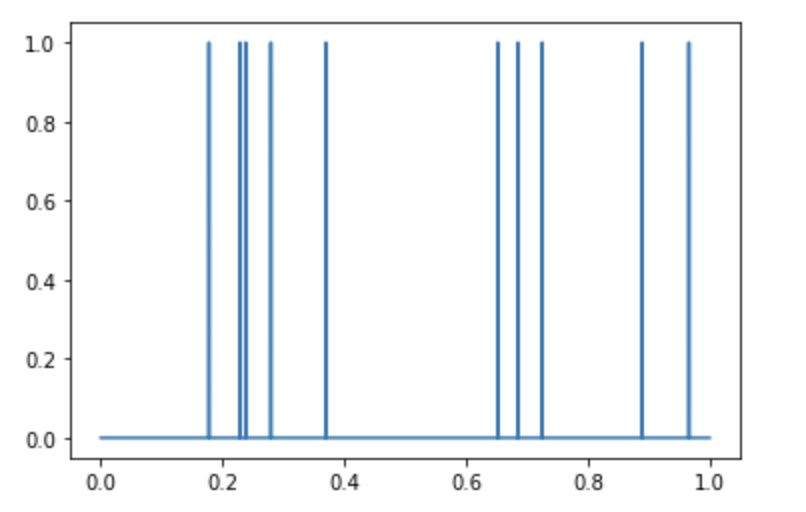
\includegraphics[width=0.75\textwidth]{18.png}
        \caption{2}
        \label{fig:first}
\end{figure}

С более естественными звуками результаты несколько отличаются. Рассмотрим запись гобоя.

\begin{figure}[H]
        \centering
        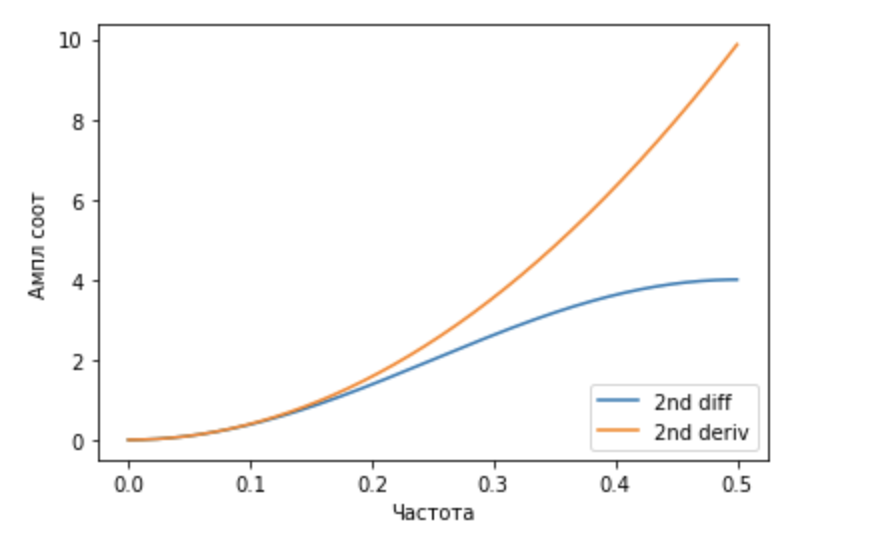
\includegraphics[width=0.75\textwidth]{19.png}
        \caption{2}
        \label{fig:first}
\end{figure}

Здесь все углы установлены в ноль:

\begin{figure}[H]
        \centering
        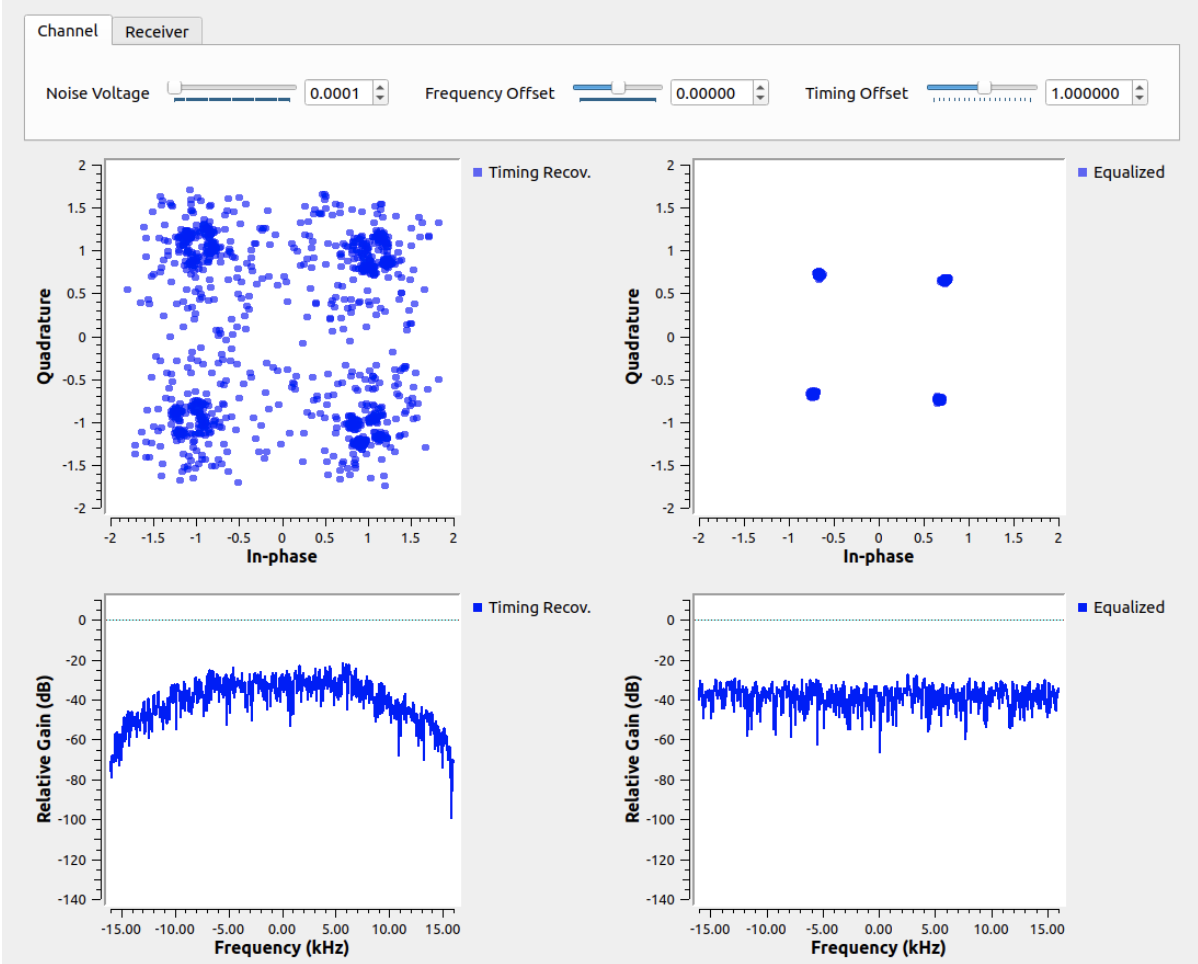
\includegraphics[width=0.75\textwidth]{20.png}
        \caption{2}
        \label{fig:first}
\end{figure}

Здесь все углы повернуты на 1 радиан: 

\begin{figure}[H]
        \centering
        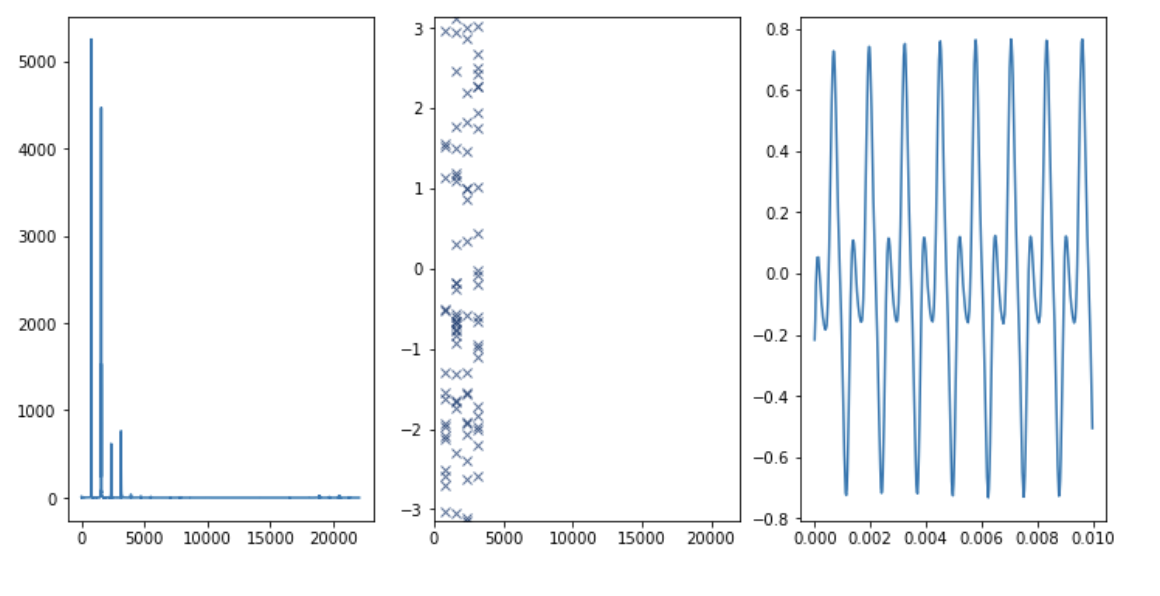
\includegraphics[width=0.75\textwidth]{21.png}
        \caption{2}
        \label{fig:first}
\end{figure}

Здесь все углы принимают случайные значения.

\begin{figure}[H]
        \centering
        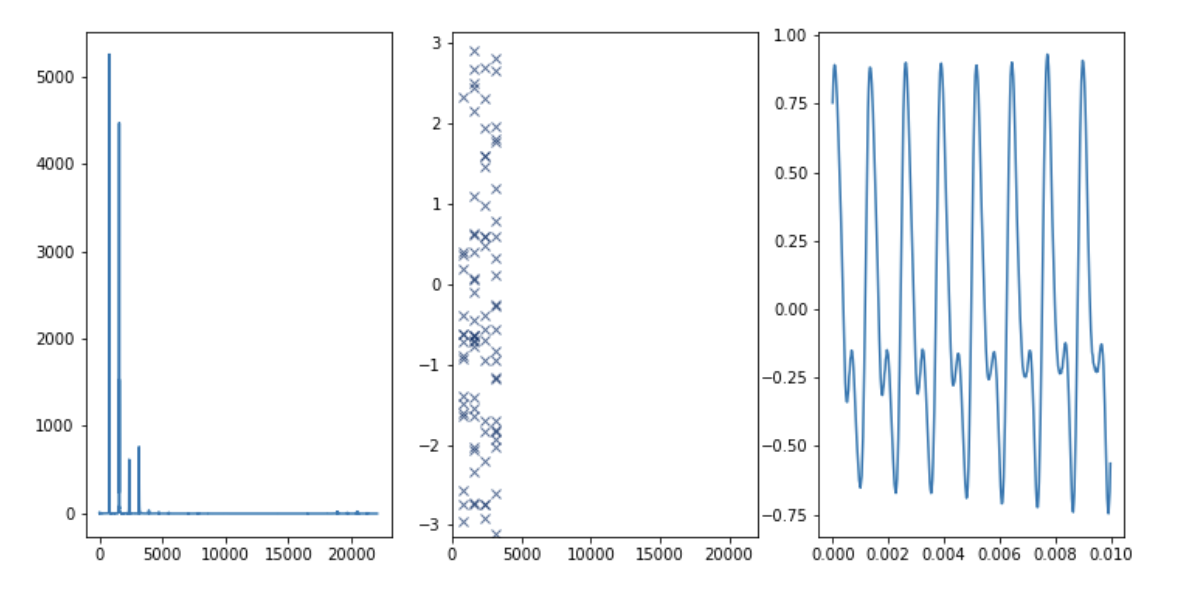
\includegraphics[width=0.75\textwidth]{22.png}
        \caption{2}
        \label{fig:first}
\end{figure}

Установка углов в ноль понижает уровень громкости, поворот углов на радиан не вызвал особых изменений. В случае со случайными значениями появились эффекты ревебрации.

Проделаем те же операции с небольшим сегментом звука саксофона:

\begin{figure}[H]
        \centering
        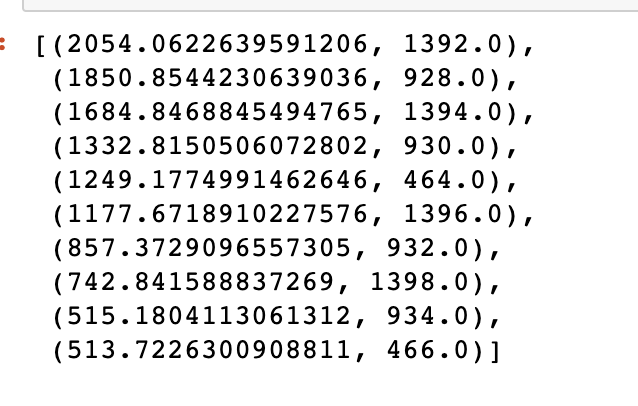
\includegraphics[width=0.75\textwidth]{23.png}
        \caption{2}
        \label{fig:first}
\end{figure}

Здесь все углы установлены в ноль:

\begin{figure}[H]
        \centering
        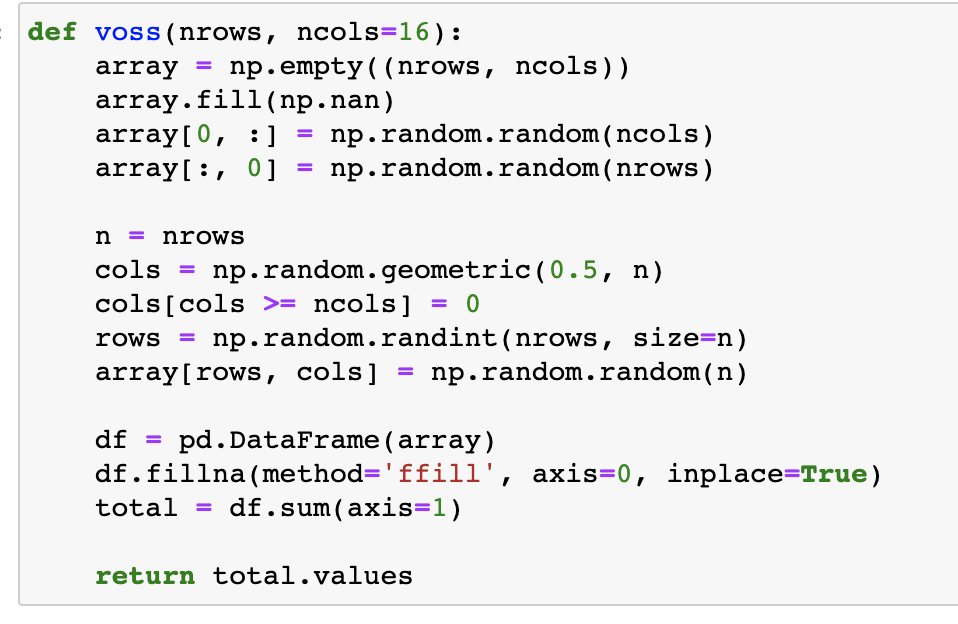
\includegraphics[width=0.75\textwidth]{24.png}
        \caption{2}
        \label{fig:first}
\end{figure}

Здесь все углы повернуты на 1 радиан: 

\begin{figure}[H]
        \centering
        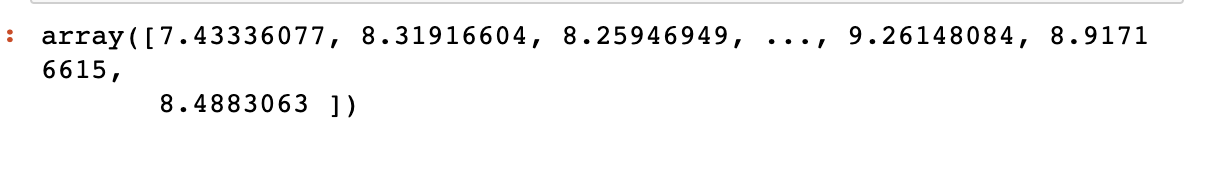
\includegraphics[width=0.75\textwidth]{25.png}
        \caption{2}
        \label{fig:first}
\end{figure}

Здесь все углы принимают случайные значения.

\begin{figure}[H]
        \centering
        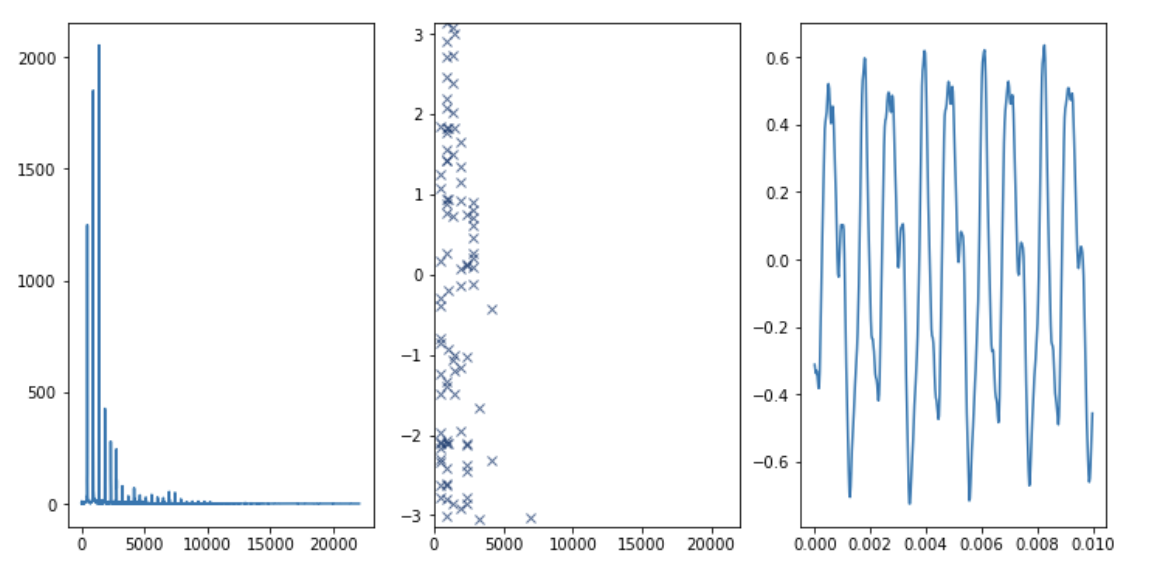
\includegraphics[width=0.75\textwidth]{26.png}
        \caption{2}
        \label{fig:first}
\end{figure}

Таким образом после всех преобразований можно сделать вывод, что при установлении значений углов в 0 звук теряет небольшую часть громкости и становится тише, в случае с поворотом углом звук не изменяется, а при установлении случйных значений мы начинаем слышать шумы которые снижают качество звука (личная оценка)

Саксофон отличается от других звуков тем, что основной компонент не является доминирующим. Для подобных звуков ухо использует что-то вроде автокорреляции в дополнение к спектральному анализу, и возможно, что этот вторичный режим анализа более чувствителен к фазовой структуре.

\end{document}